\hypertarget{section-quality-scenarios}{%
\section{9 Quality Requirements}\label{section-quality-scenarios}}

\textbf{Contents}

This section details the quality requirements for the Webshop system, focusing on performance, security, usability, maintainability, and reliability. It includes a quality tree to prioritize these attributes and quality scenarios to make them concrete and measurable, covering both critical goals (e.g., security) and lower-priority ones (e.g., reliability).

\textbf{Motivation}

Quality requirements are essential for the Webshop to meet user expectations, ensure reliable operation, and support future growth. They guide architectural decisions about cloud infrastructure, payment integration, and user interface design, ensuring the system is secure, performant, and user-friendly for users.

\hypertarget{_quality_tree}{%
\subsection{Quality Tree}\label{_quality_tree}}

\textbf{Contents}
The quality tree organizes the Webshop’s quality attributes, starting with ‘Quality’ as the root and branching into categories like Performance, Security, Usability, Maintainability, and Reliability, with sub-attributes and priorities linked to quality scenarios. It reflects both normal operating conditions and peak demand scenarios to ensure comprehensive coverage.

\textbf{Motivation}
The quality tree provides a structured overview and prioritization of the Webshop’s quality requirements, helping Developers focus on critical aspects like security and performance while addressing secondary goals like usability and system reliability. It enables architects to evaluate and design the system effectively, linking to detailed scenarios for validation.

\textbf{Form}
The quality tree is presented as a hierarchical diagram, with ‘Quality’ at the top-left, branching horizontally into categories and sub-attributes, each with priorities (High, Medium, Low) and references to corresponding quality scenarios in the Quality Scenarios section.

\begin{figure}[h]
  \centering
  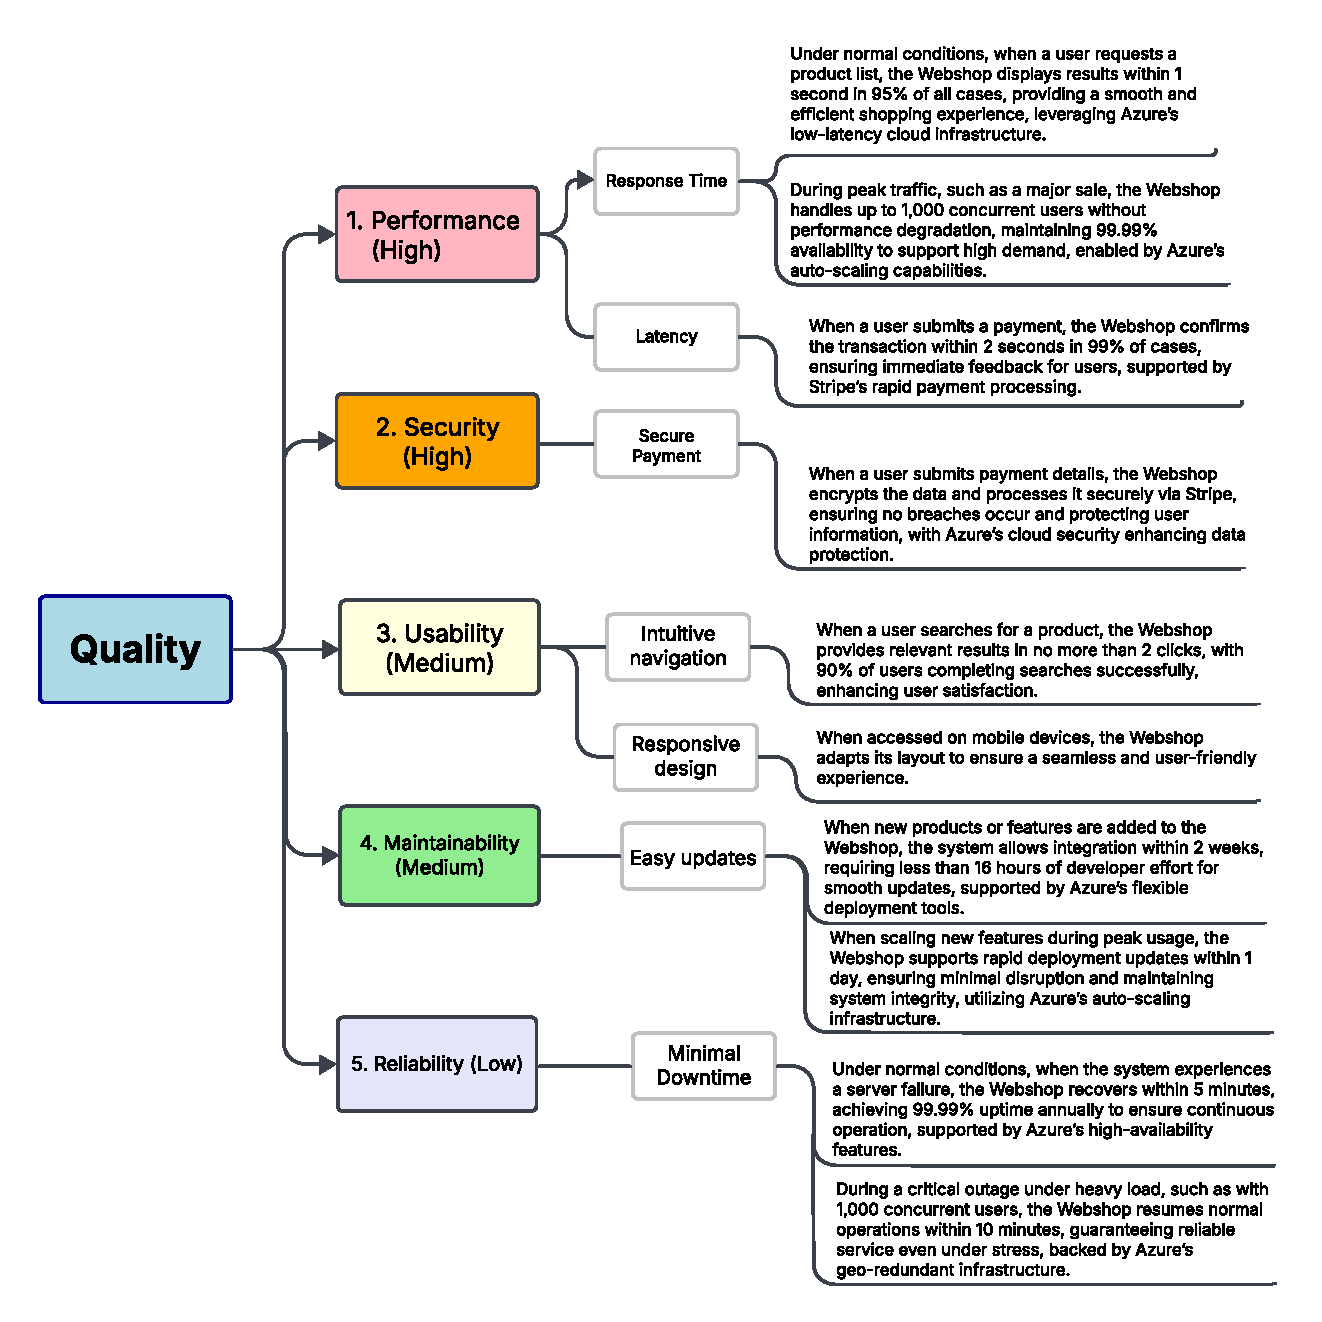
\includegraphics[width=0.9\textwidth]{images/quality-tree.pdf}
  \caption{Quality Tree for the Webshop System}
  \label{fig:webshop-quality-tree}
\end{figure}

\hypertarget{_quality_scenarios}{%
\subsection{Quality Scenarios}\label{_quality_scenarios}}

\textbf{Contents}

This subsection provides concrete quality scenarios for the Webshop, detailing runtime responses to stimuli (usage scenarios) and system modifications (change scenarios), with measures and priorities linked to the quality tree. It includes scenarios for both normal conditions and peak demand to ensure robust system performance.

\textbf{Motivation}

Quality scenarios make the Webshop’s quality requirements tangible, allowing architects to design and test for performance, security, usability, and reliability. They ensure the system meets user expectations, supports cloud-based operations and payment integration, and can be evaluated for trade-offs, providing clarity for Developers in development and evaluation.

\textbf{Form}

Quality scenarios are presented in a tabular format, with columns for scenario type, stimulus, response, measure, and priority, corresponding to leaves in the quality tree.

\begin{table}[h]
  \centering
  \renewcommand{\arraystretch}{1.2} 
  \setlength{\tabcolsep}{4pt} 
  \resizebox{\textwidth}{!}{ 
      \begin{tabular}{|p{3cm}|p{3cm}|p{4cm}|p{3cm}|c|}
          \hline
          \textbf{Scenario Type} & \textbf{Stimulus} & \textbf{Response} & \textbf{Measure} & \textbf{Priority} \\
          \hline
          Usage (Performance)  & User requests a product list & System displays products within 1 second & 95\% of requests complete in <1 second & High \\
          \hline
          Change (Performance)  & Traffic spikes during a sale & System handles 1,000 concurrent users & 99\% availability during peak load & High \\
          \hline
          Usage (Performance)  & User submits payment & System confirms transaction within 2 seconds & 99\% of transactions complete in <2 seconds & High \\
          \hline
          Usage (Security)  & User submits payment details & System encrypts data and processes via Stripe & Data encrypted with TLS 1.2, no breaches & High \\
          \hline
          Usage (Usability)  & User searches for a product & System shows relevant results in 2 clicks & 90\% of users complete searches successfully & Medium \\
          \hline
          Usage (Usability)  & User accesses Webshop on mobile & System adapts layout for mobile devices & 95\% of mobile users report satisfaction & Medium \\
          \hline
          Change (Maintainability)  & New products or features are added & System integrates within 2 weeks & Integration completed with <16 hours effort & Medium \\
          \hline
          Change (Maintainability)  & Scaling new features during peak usage & System integrates updates within 1 day & Integration completed with <24 hours effort & Medium \\
          \hline
          Usage (Reliability)  & System experiences server failure & System recovers within 5 minutes & 99.9\% uptime annually & Low \\
          \hline
          Usage (Reliability)  & System outage under heavy load & System resumes normal operations within 10 minutes & 99.9\% uptime during peak load & Low \\
          \hline
      \end{tabular}
  }
  \caption{Quality Scenarios for the Webshop System}
  \label{tab:webshop-quality-scenarios}
\end{table}


\end{document}